\chapter{Introduction}
\label{ch:intro}
%-------------------------------------------------------
This project implemented basic image processing functionality using OpenCV. These included loading and displaying the original image, generating histograms of both the original and previewed images, and interactive scroll bars to dynamically adjust brightness and contrast. It included a saving feature to save the processed image for later use with your adjusted settings intact upon restart. The implementation gave hands-on experience with image manipulation, displaying histograms, and the development of interactive interfaces focused on practical computer vision applications.
%%%%%%%%%%%%%%%%%%%%%%%%%%%%%%%%%%%%%%%%%%%
%%% SUBSECTION NAME
%%%%%%%%%%%%%%%%%%%%%%%%%%%%%%%%%%%%%%%%%%%%%%%%%%%%%

\section{Loading The Given Image And Intial Histograms On The Screen}
To begin, we must load the given information and histograms into our program.
\begin{minted}[frame=single,framesep=10pt]{python}
iimageLeft = cv2.imread('dog.bmp')
adjusted = imageLeft.copy()

#make window
cv2.namedWindow(WINDOWNAME)

#show default image
stacked = np.hstack((imageLeft, adjusted))

#generate scaled histograms for the original image
histleft = generateScaledHistogram(imageLeft)
histadjusted = generateScaledHistogram(adjusted)

#stack the images and histograms initially
stacked = np.vstack((stacked, np.hstack((histleft, histadjusted))))

#show the stacked image with histograms
cv2.imshow(WINDOWNAME, stacked)
\end{minted}
Initially, we load the image 'dog.bmp' into a variable called imageLeft, this will be our reference image for performing filtering. Then we duplicate the image so that we have one to filter, this will be called adjusted. now we start up the window so that we can have an active display. Then we create a stack that allows us to display the two images side by side, assign it to one variable. We can then generate the histograms using the functions which return images of the completed histograms.(See Below for Histogram generation Function) After generating those two images we can stack them horizontally and then vertically with the raw images to get our final display of 2 images and 2 histograms.

The Histogram generation function is shown below.
\begin{minted}[frame=single,framesep=10pt]{python}
def generateScaledHistogram(image):
    #convert the image to grayscale for histogram calculation
    gray = cv2.cvtColor(image, cv2.COLOR_BGR2GRAY)

    hist = cv2.calcHist([gray], [0], None, [256], [0, 256])

    #normalize the histogram to fit it in the image window
    hist = hist / hist.max()  

    #create a blanck histogram so we can fill it with the data
    histheight = image.shape[0]
    histwidth = 256 
    histimage = np.zeros((histheight, histwidth, 3), dtype=np.uint8)

    #draw
    for i in range(1, 256):
        cv2.line(histimage,(i-1, histheight - int(hist[i-1] * histheight)),
        (i, histheight - int(hist[i] * histheight)),(255, 255, 255), 1)

    #resize the histogram image to the same size as the original image
    scaled = cv2.resize(histimage, (image.shape[1], image.shape[0]))

return scaled
\end{minted}
The image is passed to the function where it is than converted to greyscale to represent in the histogram, the histogram is than generated from the image. The values are than normalized. We can than create a blank histogram with the dimensions of the original image so we can show it in the window. We can than fill the blank histogram with our normalized values from the scaled image. the scaled image is then resized and returned.
\begin{figure}[h!]
    \centering
    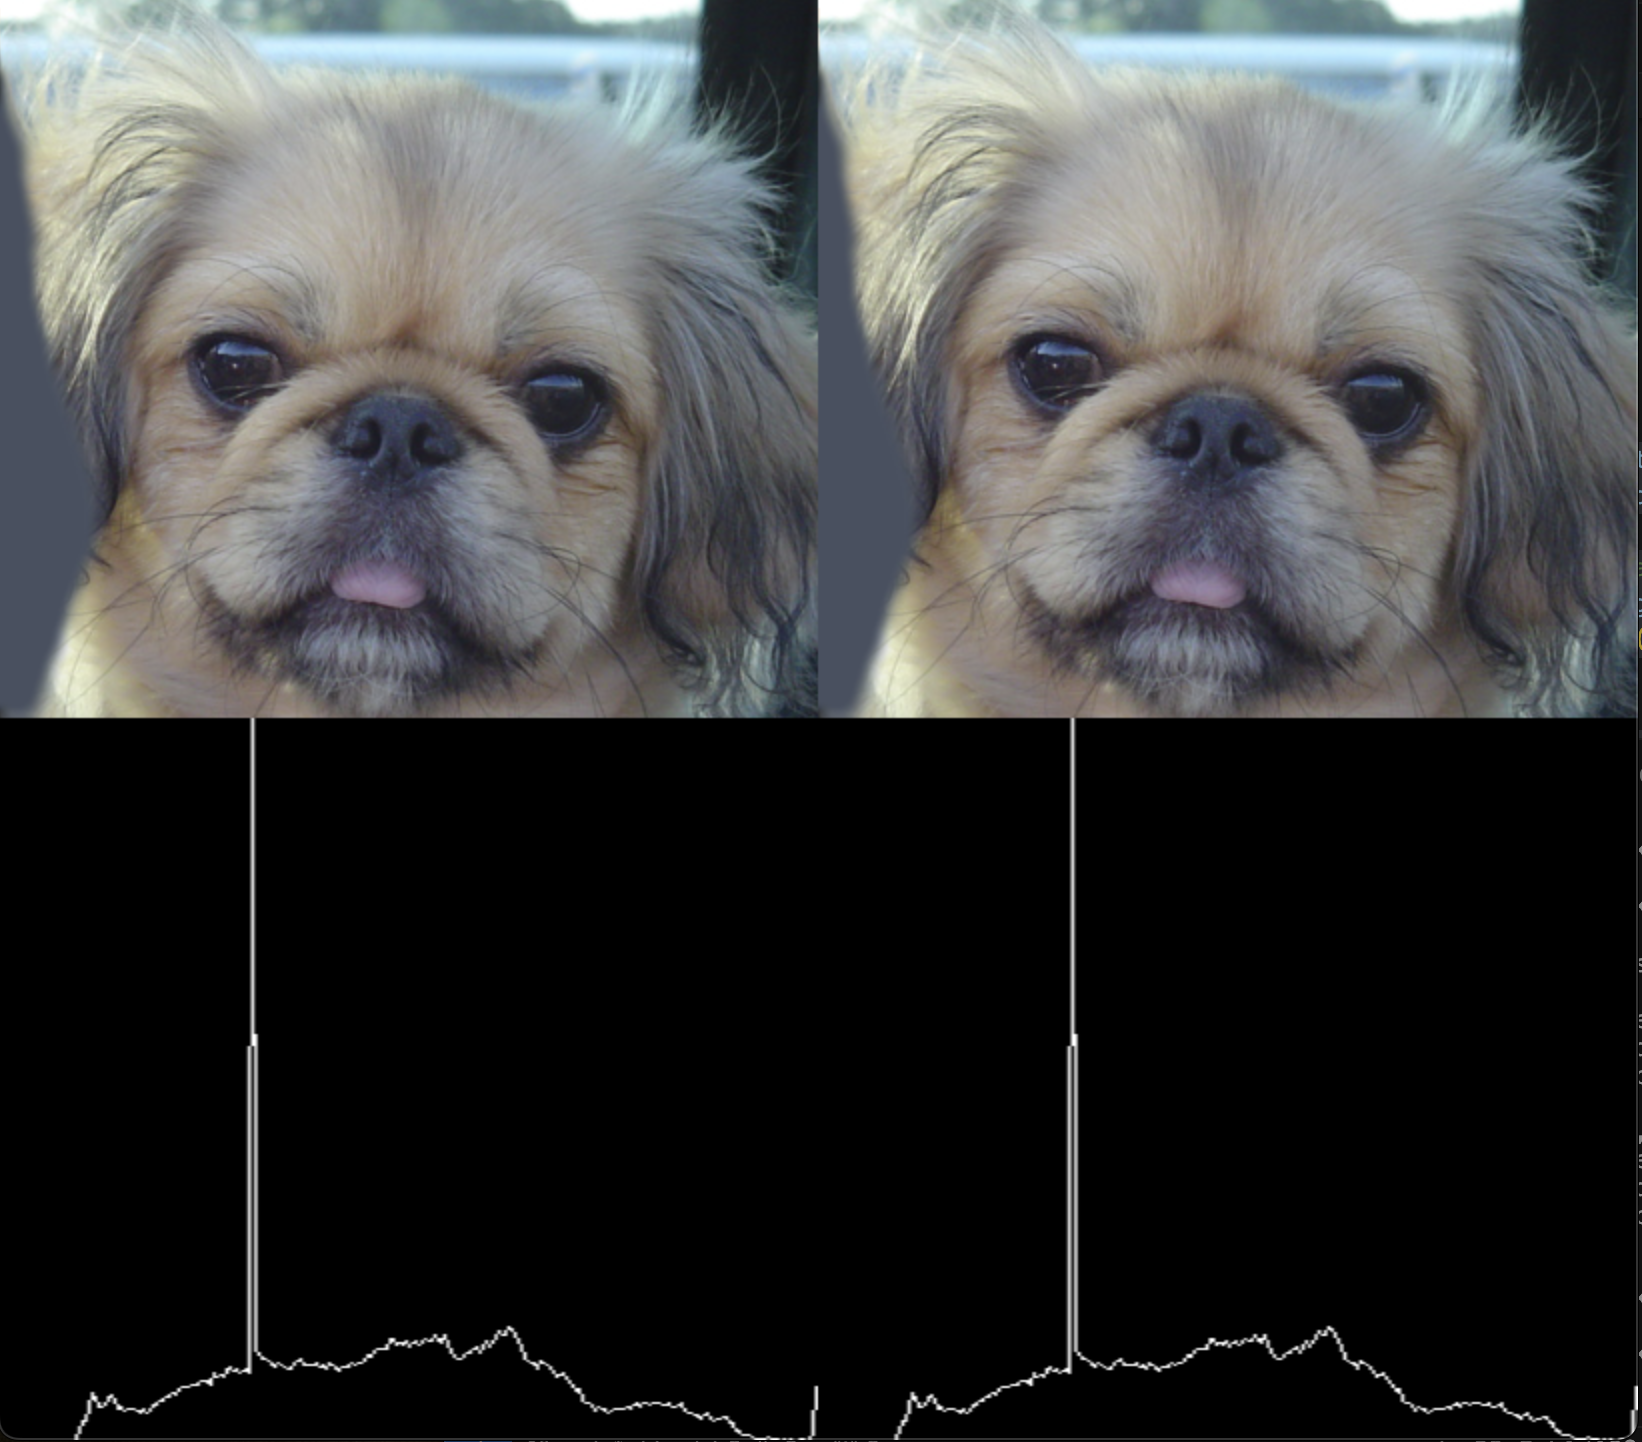
\includegraphics[width = 0.5\textwidth]{figure1.1.png}
    \caption[Just Images and Histograms]%
    {Just Images and Histograms} 
    \label{fig:exA}
\end{figure}
%%%%%%%%%%%%%%%%%%%%%%%%%%%%%%%%%%%%%%%%%%%%%%%%%%%%%
%%% SUBSECTION NAME
%%%%%%%%%%%%%%%%%%%%%%%%%%%%%%%%%%%%%%%%%%%%%%%%%%%%%
\section{Scroll Bar Implementation}
The scroll bar for controlling Brightness and Contrast for the picture was implemented fairly simply.
\begin{minted}[frame=single,framesep=10pt]{python}
#create sliderbar for brightness and contrast
cv2.createTrackbar('Brightness', WINDOWNAME, 128, 255, adjust_brightness)
cv2.createTrackbar('Contrast', WINDOWNAME, 128, 255, adjust_contrast)
\end{minted}
The createTrackbar option creates trackbars that pass the values of the trackbars into two functions. adjust brightness and adjust contrast.
\begin{minted}[frame=single,framesep=10pt]{python}
def adjust_brightness(val):
    global lastConst
    global lastBright
    global adjusted

    lastConst = val / 100

    #adjust contrast
    adjusted = cv2.convertScaleAbs(imageLeft,alpha = lastConst , 
    beta= lastBright )
    stacked = np.hstack((imageLeft, adjusted))
    
    #generate scaled histograms for original and adjusted images
    histleft = generateScaledHistogram(imageLeft)
    histadjusted = generateScaledHistogram(adjusted)
    
    #stack the images and histograms
    stacked = np.vstack((stacked, np.hstack((histleft, histadjusted))))
    
    cv2.imshow(WINDOWNAME, stacked)
\end{minted}
The function implementation is fairly simple, to adjust either the brightness or contrast we can use the function convertScaleABS adjusting the beta value in that function it will adjust the brightness of the image and if we adjust alpha we will adjust the contrast. We can then save the new image as a variable to load into the program. We than generate the histograms just like before and replace the current images with the new ones we just generated The adjust contrast function does the same but adjusts the beta value
\begin{figure}[h!]
    \centering
    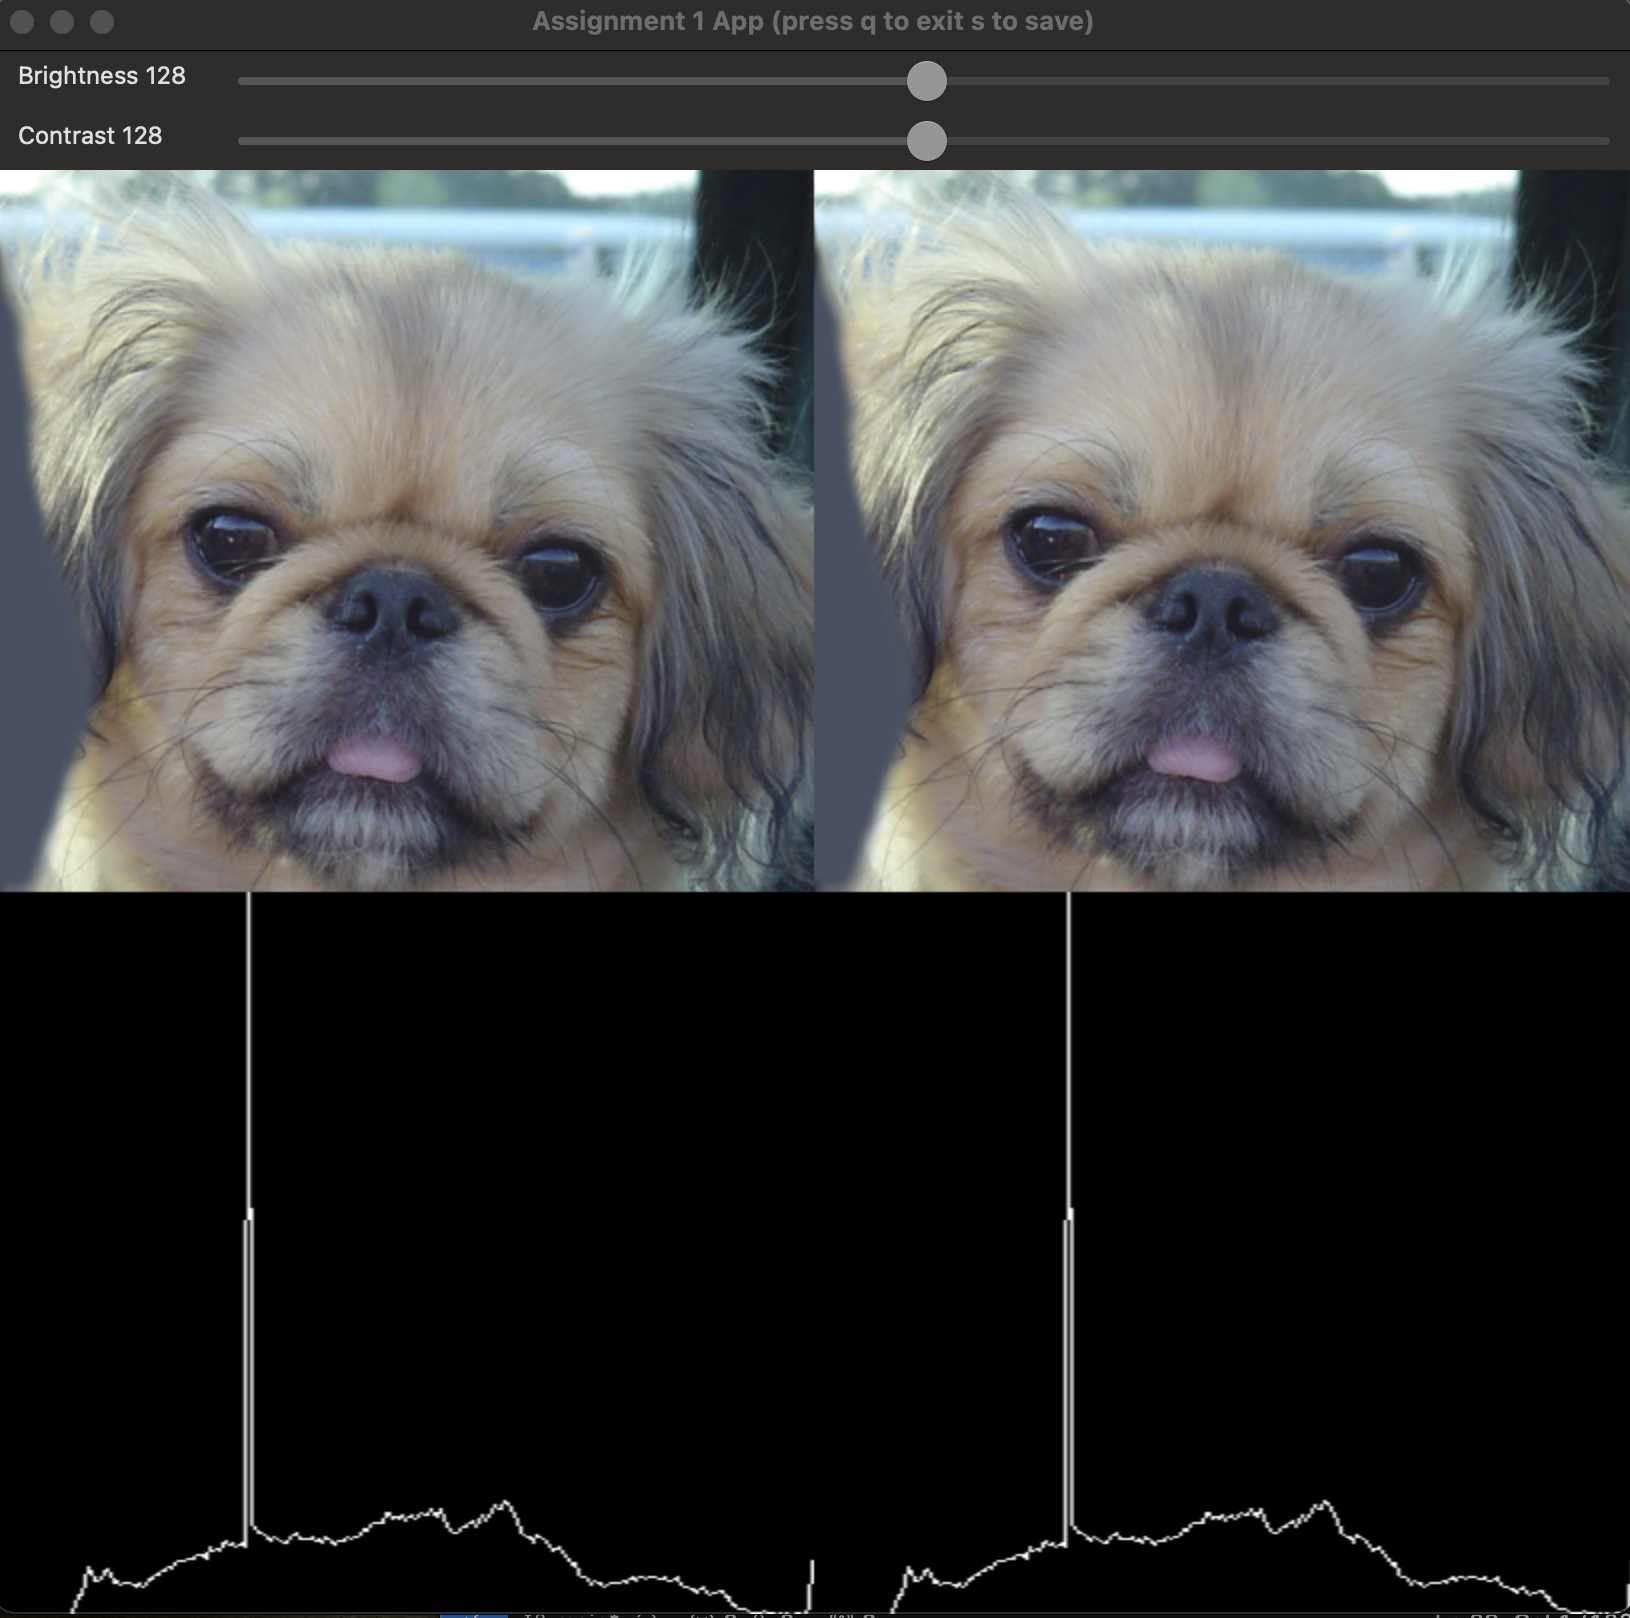
\includegraphics[width = 0.8\textwidth]{figure1.2.png}
    \caption[Added Scroll Bars]%
    {Added Scroll Bars} 
\end{figure}
%%%%%%%%%%%%%%%%%%%%%%%%%%%%%%%%%%%%%%%%%%%%%%%%%%%%%
%%% SUBSECTION NAME
%%%%%%%%%%%%%%%%%%%%%%%%%%%%%%%%%%%%%%%%%%%%%%%%%%%%%
\section{Save and quit Function}
The program also features both a save and a quit funciton
\begin{minted}[frame=single,framesep=3pt]{python}
while True:
    if cv2.waitKey(1) == ord('q'):
        break
    if cv2.waitKey(1) == ord('s'):
        #save
        cv2.imwrite('dog-modified.bmp', adjusted)
        
        #reload the saved image
        as the new 'imageLeft' for further adjustments
        imageLeft = cv2.imread('dog-modified.bmp')
        adjusted = imageLeft.copy()
        
        #update the display
        stacked = np.hstack((imageLeft, adjusted))
        hist_left = generateScaledHistogram(imageLeft)
        hist_adjusted = generateScaledHistogram(adjusted)
        stacked_with_hist = np.vstack((stacked,
        np.hstack((hist_left, hist_adjusted))))
        cv2.imshow(WINDOWNAME, stacked_with_hist)
        \end{minted}
When the user clicks S the adjusted image on the right overwrites the image on the left and now it becomes the reference image to be adjusted. The program will also save the photo as 'dog-modified.bmp'. If the user clicks q the program will exit when restarted it will load the original loaded image
\begin{figure}[h!]
    \centering
    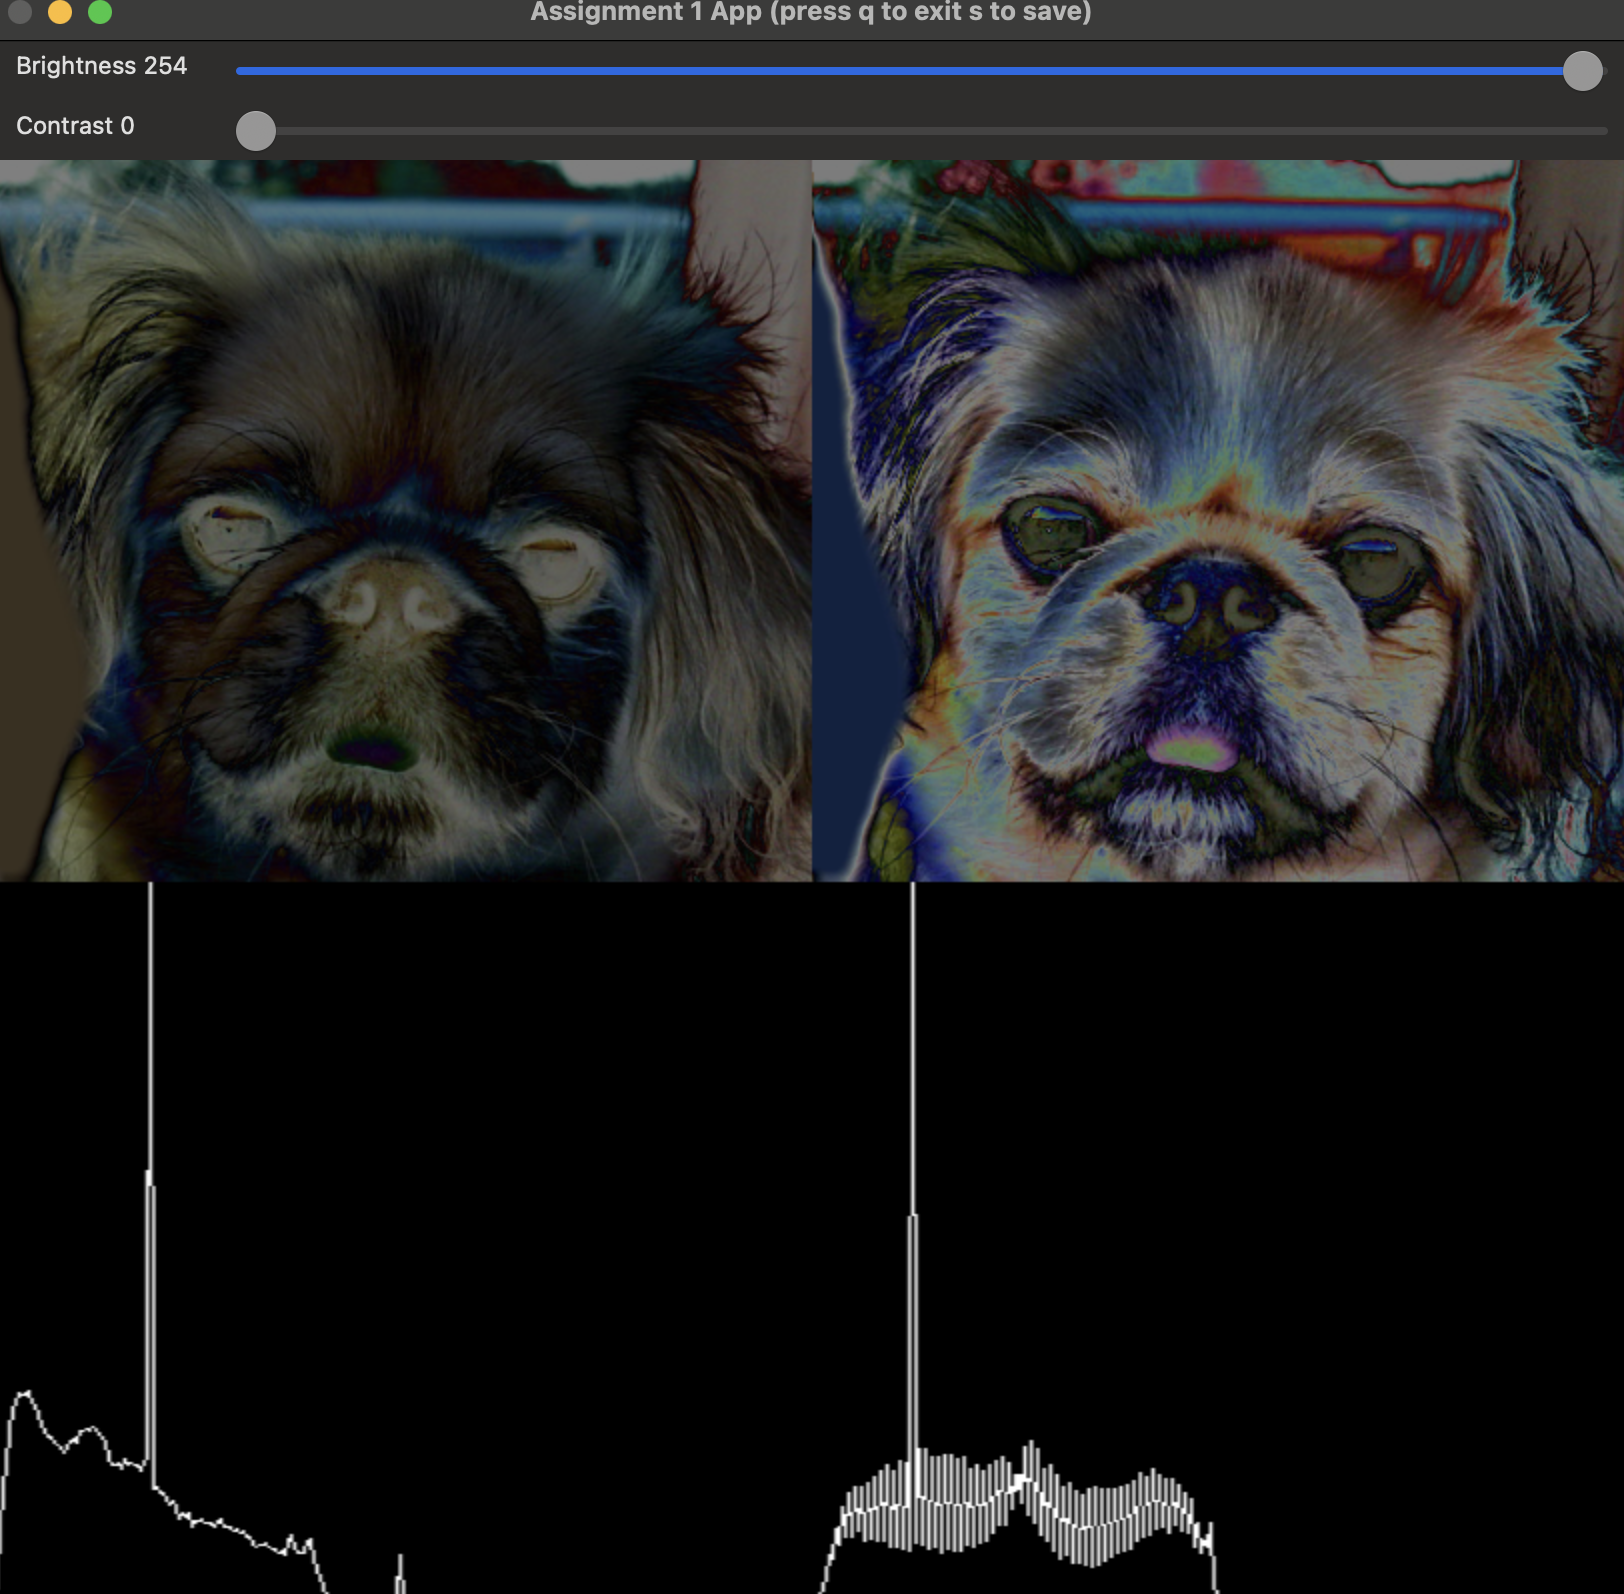
\includegraphics[width = .35\textwidth]{figure1.3.png}
    \caption[Showed Save Functionality]%
    {Showed Save Functionality} 
\end{figure}

\section{Discussion}
This computer vision homework had a fair amount in it that i had to learn about in python. First, there was the histograms. I used Matplotlib initially to create the histograms, but that was rather problematic. First of all, the histograms would show up on a different window, so it was rather hard to place them correctly on my display. Secondly, the scaling was off on the acutal plot, so it was hard to properly line up the data to the picture. Using the Histogram feature in cv2 was much better. One other significant challenge was brightness and contrast adjustment. Initially, I wasn’t normalizing the values correctly, and as a result, I was getting off results and the images were not appearing as expected. It took some time for me to identify the problem and understand that normalization was needed for the adjustments to work appropriately. Finally, I had challenges implementing the scrollbar. My initial code had the default values incorrect, and because of this, the slider was not working as expected. That scrolling was not making the values correspond correctly making precise adjustments difficult to make. Despite these difficulties, overcoming these problems really allowed me to understand concepts of computer vision and debugging techniques.